\documentclass[main.tex]{subfiles}

\begin{document}
    \begin{Proof}
        \[D = \begin{pmatrix}
            \sigma_1 & & 0\\
                 &\ddots& \\
            0 & & \sigma_k
        \end{pmatrix}\]
        \[A = UDV^T\]
        \[\Abs{A} = \Abs{D} = \sup_{x \neq 0} \frac{\Abs{D_x}}{\Abs{x}} =
        \sup_{x \neq 0} \frac{\sqrt{(\sigma_1 x_1)^2 + (\sigma_2 x_2)^2 + ... +
    (\sigma_k x_k)^2}}{\sqrt{x_1^2 + ... + x_n^2}} \]
    \end{Proof}

    \begin{task}
        Необходимо сжать изображение. Мы хотим сделать так, чтобы
        фотография занимала меньше места на компьютере. Формально, мы ищем
        матрицу, которая близка к исходной.
    \end{task}

    \begin{Proof}
        \[A \in M_{m,n}(\R) \qq m \geq n \]
        \[\hat{A} \in M_{m, n}(\R)  \qq \Abs{A - \hat{A}} \to \min \qq \rk \hat{A} \leq r\]
        Мы можем измерить объем информации рангом матрицы и хранить ЛНЗ строки и
        линейные комбинации\\
        \\
        \[A = UDV^{T} \]
        \[U = (U_1U_2)\]
        \[V = (V_1V_2)\]
        \[U_1 \in M_{m, r}(\R) \]
        \[V_1 \in M_{n, r }(\R)\]
        \[D = \begin{pmatrix}
            D_1 & 0\\
            0 & D_2
        \end{pmatrix} \qq D_1 \in M_r (\R)\]
        \[\hat{A} = U_1D_1V_1^T\]
        \[\hat{A} = U\begin{pmatrix}
            D_1 & 0 \\
            0 & 0
        \end{pmatrix} V^T\]
        \[\Abs{A - \hat{A}} = \Abs{U\begin{pmatrix}
            0 & 0 \\
            0 & D_2
            \end{pmatrix} V^T} = \Abs{\begin{pmatrix}
            0 & 0\\
            0 & D_2
        \end{pmatrix}} = \sigma_{r + 1} \]
        \[B \in M_{m, n}(\R) \ \os{?}{\Ra} \ \Abs{A - B} \geq \sigma_{r + 1} \]
        \[\rk B = r\]
        \[\rk B = r \ \Ra \ B = XY^T, \qq X \in M_{m, r}(\R) \q Y \in M_{n, r}(\R)  \]
        Матрица $Y$ образована из ЛНЗ строк из $B$. Каждая строка $B$ записывается как ЛК
        этих строчек. $X$ --- матрица коэфф.
        \[\mathcal{Y} \text{ --- линейная оболочка столбцов } Y \q \text{(в $\R^n$)}\]
        \[\dim \mathcal{Y} \leq r\]
        Можно взять орт. дополнение
        \[\Ra \dim \mathcal{Y}^\perp \geq n - r\]
        \[\mathcal{\hat{V}} \text{ --- линейная оболочка первых } r + 1 \text{ столбцов } V
        \qq(\text{ в } \R^n)\]
        \[\dim \mathcal{\hat{V}} = r + 1\]
        У них есть нетрив. пересеч. по формуле размерностей подрв-в
        \[\Ra \exists  \ w \in \mathcal{\hat{V}} \cap \mathcal{Y}^{\perp} \qq w \neq 0\]
        \[\Abs{w} = 1\]
        \[w \in \mathcal{Y}^\perp \ \Ra \ Y^T_w = 0\]
        \[w \in \mathcal{\hat{V}} \ \Ra \ w = V \begin{pmatrix}
            \gamma_1\\
            \vdots\\
            \gamma_{r + 1}\\
            0\\
            \vdots\\
            0
        \end{pmatrix}\]
        \[\Abs{A - B}^2 \geq \Abs{(A - B)w}^2 = \Abs{Aw}^2 = \Abs{UDV^{T}V \begin{pmatrix}
            \gamma_1\\
            \vdots\\
            \gamma_{r + 1}\\
            0\\
            \vdots\\
            0
        \end{pmatrix}}^2 = \Abs{D \begin{pmatrix}
            \gamma_1\\
            \vdots\\
            \gamma_{r + 1}\\
            0\\
            \vdots\\
            0
        \end{pmatrix}}^2\]
        \[= \sigma_1^2 \gamma_1^2 + ... + \sigma_{r + 1}^2 \gamma_{r + 1}^2 \geq
        \sigma_{r + 1}^2 \]
        \[1 = \Abs{w} = \Abs{V \begin{pmatrix}
            \gamma_1\\
            \vdots\\
            \gamma_{r + 1}\\
            0\\
            \vdots\\
            0
        \end{pmatrix}} = \Abs{\begin{pmatrix}
            \gamma_1\\
            \vdots\\
            \gamma_{r + 1}\\
            0\\
            \vdots\\
            0
        \end{pmatrix}} = \sqrt{\gamma_1^2 + ... + \gamma_{r + 1}^2} \]
    \end{Proof}

    \subsection{Аффинное подпространство с минимальной суммой квадратов расстояний до данного набора точек (и максимальной дисперсией их проекций). Формулировка задачи минимизации и сдвиг в центр масс}

    \begin{task}
        В $n$ --- мерном пр-ве есть набор точек и нам нужно найти подпр-во
        заданной размерности,
        которое приближает этот набор точек. Что значит приближает? Это наилучшая
        аппроксимакция этих точек. Берем точки и их проекции. Складываем расстояния в
        квадрате для каждой точки. \\ %%кажется, тут проблемы с русским языком
        %рисунок1
        \begin{figure}[H]
            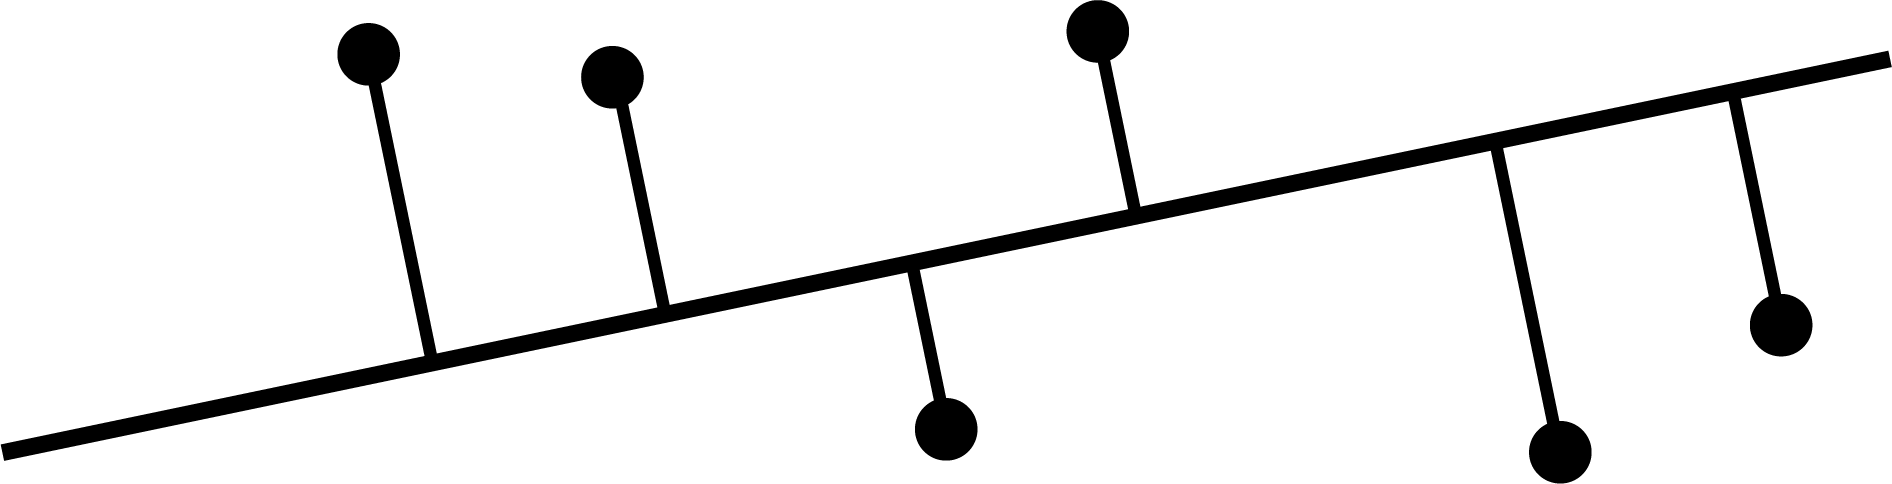
\includegraphics[width=7cm]{pics/11_1.png}
            \centering
            \caption{прямая, которая аппроксимирует точки}
        \end{figure}
        Дисперсия --- сумма квадратов отклонений от среднего значения (центр массы)
        \[x_1, ..., x_m \in \R^n\]
        \[\dim L = k \qq L = \ <\us{\text{ортнорм}}{u_1, ..., u_k}>\]
        \[\pr_L x = \sum_{i = 1}^k  (u_i, x)u_i = \begin{pmatrix}
            u_1 &...& u_k
        \end{pmatrix} \begin{pmatrix}
            (u_1, x)\\
            \vdots\\
            (u_k, x)
        \end{pmatrix} =\]
        \[(U = (\begin{pmatrix}
            u_1 &...& u_k
        \end{pmatrix}) \in M_{n, k}(\R))\]
        \[ = \begin{pmatrix}
            u_1 & ... & u_k
        \end{pmatrix} \begin{pmatrix}
            u_1^T\\
            \vdots\\
            u_k^T
        \end{pmatrix}x = UU^Tx\]
        \[U^TU = I_k\]
        \[\min \sum_{i = 1}^m \Abs{(I_n - UU^T)(x_i - u_0)}^2 \]
        \[U \in M_{n, k} (\R) \]
        \[U^TU = I_k\]
        \[u_0 \in \R^n\]
        Любое подпр-во проходит через ноль, но мы хотим избавиться от этого ограничения.
        Мы можем перенести наше под-прво. $u_0$ --- вектор сдвига.\\
        Или мы сдвигаем все точки на $u_0$.
    \end{task}

    \subsection{Аффинное подпространство с минимальной суммой квадратов расстояний до данного набора точек (и максимальной дисперсией их проекций). Окончание доказательства}

    \begin{Proof}[решение]
        \[X = \begin{pmatrix}
            x_1^T\\
            \vdots\\
            x_m^T
        \end{pmatrix} \in M_{m, n}(\R) \]
        \[\overline{x} = \frac{1}{m}\sum_{i = 1}^m x_i  \text{  --- центр масс}\]
        \[\widetilde{X} = X - \begin{pmatrix}
            \overline{x}^T\\
            \vdots\\
            \overline{x}^T
        \end{pmatrix} \text{ центрированная матрица} \q \in M_{m, n} (\R) \]
        \[\widetilde{X}^T\widetilde{X} \in M_{n} (\R) \]
        У этой матрицы есть система из ортонорм с.в. А соотв. с.ч. вещ. неотр.\\
        Упорядочим с.в. по величине с.ч.\\ Берем первые $k$ с.в., где $k $ --- размер
        нужного подпр-ва\\
        Нужно взять $u_0 = \overline{x}$
    \end{Proof}

    \begin{theorem}
        Такая задача о минимизации имеет след. решение. Взять $u_0 = \overline{x}$\\
        Взять в качестве $U$ матрицу, сост из первых k веторов матрицы $\widetilde{X}^T
        \widetilde{X}$, упорядоч. по собс. числу
    \end{theorem}

    \begin{Lemma}
        \[\frac{1}{m}\sum_{k = 1}^m \Abs{y_i - b}^2 = \frac{1}{m}\sum_{i = 1}^m
        \Abs{y_1 - \overline{y}}^2 + \Abs{\overline{y} - b}^2\]
        \[\overline{y} = \frac{1}{m} \sum_{i = 1}^m y_i \]
    \end{Lemma}

    \begin{Proof}
        \[\frac{1}{m} \sum \Abs{y_1 - b}^2 = \frac{1}{m}\sum \Abs{(y_1 - \overline{y}) +
        (\overline{y} - b)}^2 = \]
        \[= \frac{1}{m} \sum \Abs{y_1 - \overline{y}}^2
        + \Abs{\overline{y} - b}^2 + \frac{2}{m}\sum_{i = 1}^m (y_1 - \overline{y}, \overline{y} - b)  =\]
        \[= \frac{1}{m}\sum \Abs{y_1 - \overline{y}}^2 + \Abs{\overline{y} - b}^2 +
        \frac{2}{m}(\us{= 0 }{\sum_{i = 1}^m (y_i - \overline{y}),\ \overline{y} - b} )\]
    \end{Proof}
\end{document}
